\subsection{1c}

\lstinputlisting{p1c.py}
Next is the KS test. For this, I am unsure where I went wrong because
I followed the slides but to no avail. With time constraints, I was not
able to figure it out. Figures are plotted below. One obvious explanation
is that my distribution does not fit a Gaussian. I am unsure of potential
(and likely) bugs in my code.
\begin{figure}[h!]
    \centering
    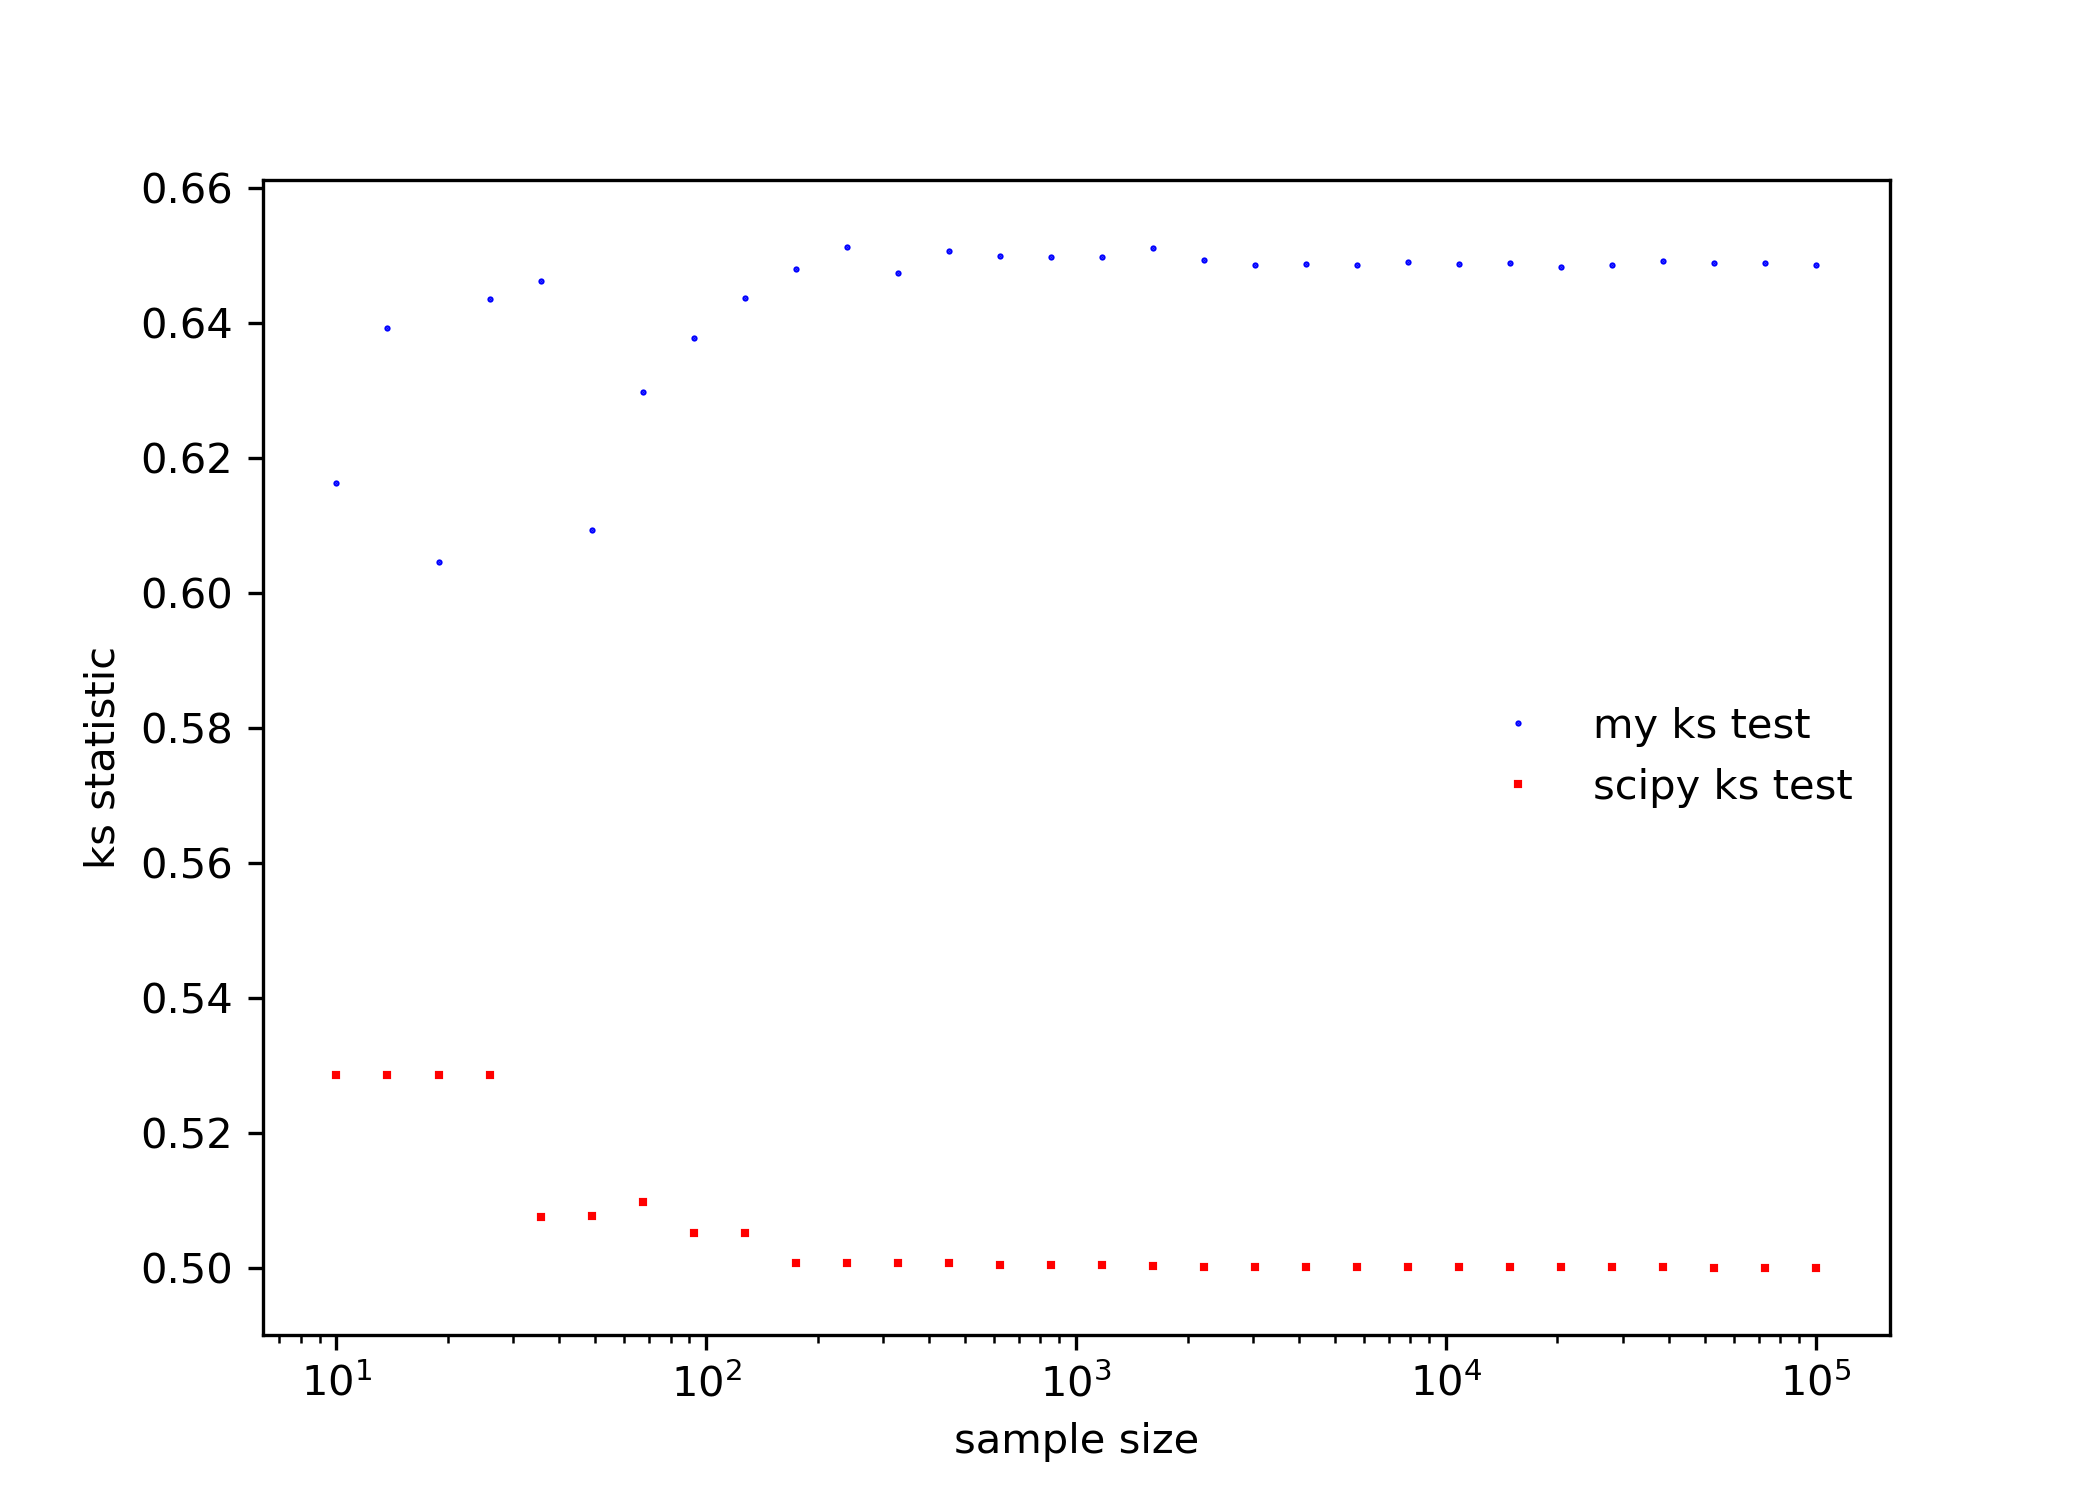
\includegraphics[width=0.9\linewidth]{./plots/ks_stat.png}
    \caption{$1$ million random numbers plotted.}
    \label{p1c1}
\end{figure}

\begin{figure}[h!]
    \centering
    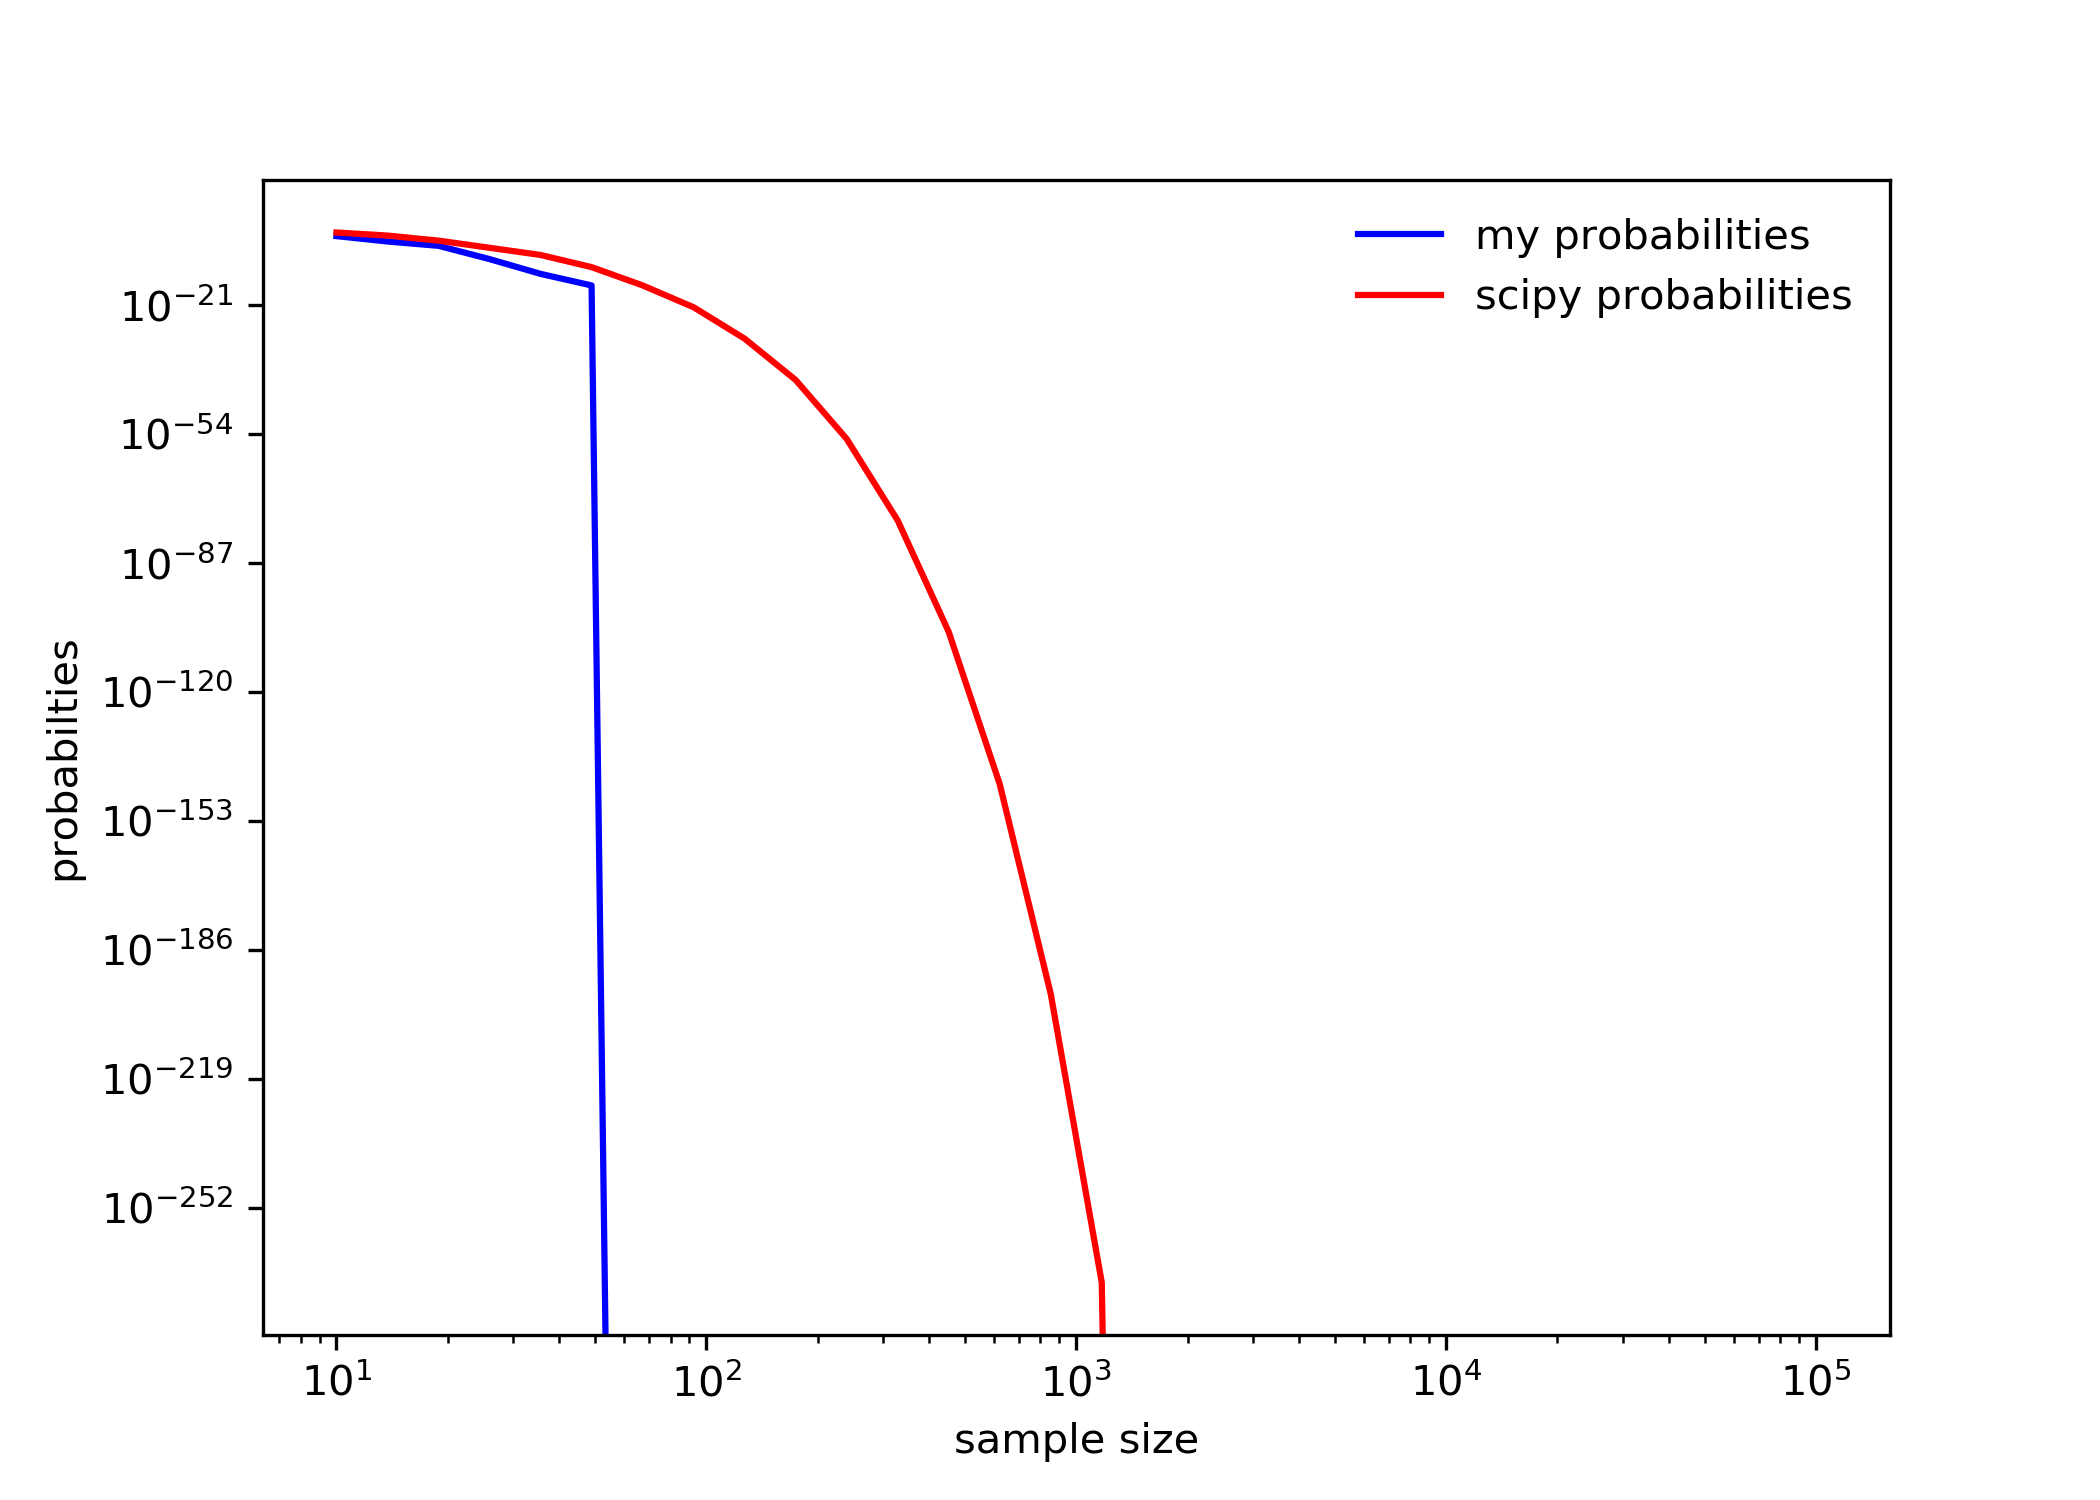
\includegraphics[width=0.9\linewidth]{./plots/ks_prob.png}
    \caption{$1$ million random numbers plotted.}
    \label{p1c2}
\end{figure}

